% \iffalse
\let\negmedspace\undefined
\let\negthickspace\undefined
\documentclass[beamer]{IEEEtran}
\usepackage{cite}
\usepackage{amsmath,amssymb,amsfonts,amsthm}
\usepackage{algorithmic}
\usepackage{graphicx}
\usepackage{textcomp}
\usepackage{xcolor}
\usepackage{txfonts}
\usepackage{listings}
\usepackage{enumitem}
\usepackage{mathtools}
\usepackage{gensymb}
\usepackage{comment}
\usepackage[breaklinks=true]{hyperref}
\usepackage{tkz-euclide} 
\usepackage{listings}
\usepackage{gvv}                                        
\def\inputGnumericTable{}                                 
\usepackage[latin1]{inputenc}                                
\usepackage{color}                                            
\usepackage{array}                                            
\usepackage{longtable}                                       
\usepackage{calc}                                             
\usepackage{multirow}                                         
\usepackage{hhline}                                           
\usepackage{ifthen}                                           
\usepackage{lscape}
\usepackage[export]{adjustbox}

\newtheorem{theorem}{Theorem}[section]
\newtheorem{problem}{Problem}
\newtheorem{proposition}{Proposition}[section]
\newtheorem{lemma}{Lemma}[section]
\newtheorem{corollary}[theorem]{Corollary}
\newtheorem{example}{Example}[section]
\newtheorem{definition}[problem]{Definition}
\newcommand{\BEQA}{\begin{eqnarray}}
\newcommand{\EEQA}{\end{eqnarray}}
\newcommand{\define}{\stackrel{\triangle}{=}}
\theoremstyle{remark}
\newtheorem{rem}{Remark}
\begin{document}
\parindent 0px
\bibliographystyle{IEEEtran}

\title{Assignment\\[1ex]10.5.4-2}
\author{ee23btech11215 - Penmetsa Srikar Varma$^{}$% <-this % stops a space
}
\maketitle
\newpage
\bigskip

\renewcommand{\thefigure}{\theenumi}
\renewcommand{\thetable}{\theenumi}
\section*{Question:}
Q10) The sum of three numbers in G.P. is 56. If we subtract 1, 7, 21 from these numbers in that order, we obtain an arithmetic progression. Find the numbers.
\section*{Solution:}
{\centering
Table of Parameters\\
}
\begin{table}[h]
    \centering
    \begin{tabular}{|c|c|}
        \hline
         Input Variable & Condition\\
        \hline
         x\brak{0} & first term of AP\\
         \hline
         r & common ratio of GP\\
         \hline
         $\frac{x\brak{0}}{r},x\brak{0},x\brak{0}.r$ & three terms in GP \\
         \hline
         $\frac{x\brak{0}}{r},x\brak{0},x\brak{0}.r$ & $\frac{x\brak{0}}{r}+x\brak{0}+x\brak{0}.r=56$ \\
         \hline
          $\frac{x\brak{0}}{r}-1,x\brak{0}-7,x\brak{0}.r-21$ & form an AP \\
         \hline
          x\brak{n-1}& $n^{th}$ term of GP \\
         \hline
         $x\brak{n}\system{Z}X\brak{z}$ & z-transform of x\brak{n}\\
         \hline
    \end{tabular}
     \label{tab:t1}
\end{table}
We know that, if three numbers p,q and r are in arithmetic progression then,
\begin{equation}
\label{q1}
2q = p + r
\end{equation}
Then $n^{th}$ term of GP x\brak{n-1} is given by:\\
\begin{align}
\label{e1}
x\brak{n-1}=x\brak{0}.r^{n-1}\quad or\quad x\brak{n}=x\brak{0}.r^{n}
\end{align}
Then from given,
\[\frac{x\brak{0}}{r}+x\brak{0}+x\brak{0}.r=56\]
\[x\brak{0}.\left(\frac{1}{r}+1+r\right)=56\]
\begin{equation}
\label{q2}
x\brak{0}=\frac{56}{\left(\frac{1}{r}+1+r\right)}
\end{equation}
and from given another case following are in AP,
\[\frac{x\brak{0}}{r}-1,x\brak{0}-7,x\brak{0}.r-21\]
Then from (\ref{q1}),
\[2.(x\brak{0}-7)=\frac{x\brak{0}}{r}-1+x\brak{0}.r-21\]
\[2.x\brak{0}-14=\frac{x\brak{0}}{r}+x\brak{0}.r-22\]
\[\frac{x\brak{0}}{r}+x\brak{0}.r-2.x\brak{0}=8\]
\[x\brak{0}\left(\frac{1}{r}+r-2\right)=8\]
and from (\ref{q2})
\[\frac{56.\left(\frac{1}{r}+r-2\right)}{\left(\frac{1}{r}+1+r\right)}=8\]
\[7\left(\frac{1}{r}+r-2\right)=\left(\frac{1}{r}+1+r\right)\]
\[\frac{6}{r}+6.r-15=0\]
\[6.r^2-15.r+6=0=2.r^2-5.r+2\]
\[(2.r-1).(r-2)=0\]
\begin{equation}
\label{q3}
r=\frac{1}{2},2
\end{equation}
so from (\ref{q2}),
\[x\brak{0}=16\]
Then from (\ref{e1}),
\begin{align}
    \label{a11}
    x\brak{n}=16.2^{n}=2^{n+4}\qquad for \brak{r=2}
\end{align}
\begin{align}
    \label{a12}
    x\brak{n}=16.\left(\frac{1}{2}\right)^{n}=2^{4-n}\quad for \brak{r=\frac{1}{2}}
\end{align}\\\\

\begin{figure}[h]
    \centering
    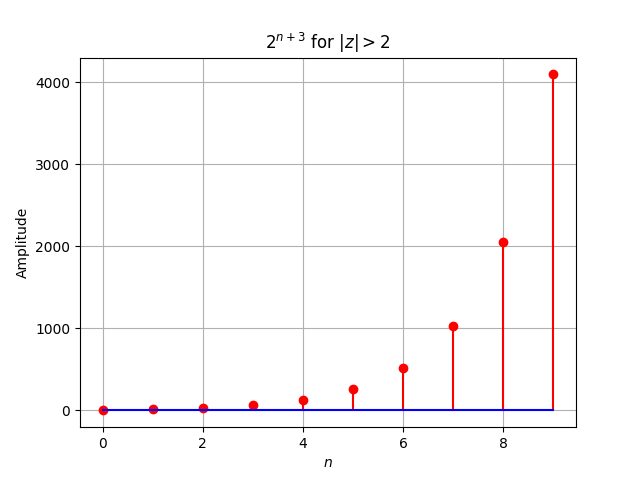
\includegraphics[scale=0.60]{py_1.png}
    \label{fig:enter-label}
\end{figure}

\begin{figure}[h]
    \centering
    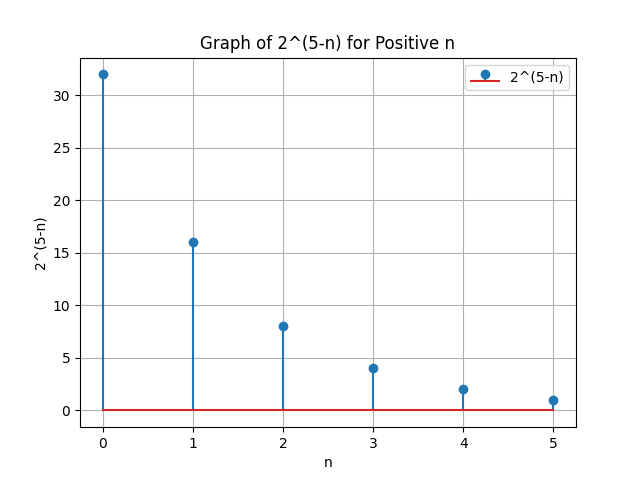
\includegraphics[scale=0.60]{py_2.png}
    \label{fig:enter-label}
\end{figure}

We know that Z-Transform of x\brak{n} is given by:
\begin{align}
\label{a13}
    X\brak{z}=\sum_{k=-\infty}^{\infty} x\brak{k}.z^{-k}
\end{align}
where, we assume that x\brak{k}=0   for \brak{k<0}\\
\brak{\ref{a13}} modify as follows:
\begin{align}
\label{a14}
    X\brak{z}=\sum_{k=0}^{\infty} x\brak{k}.z^{-k}
\end{align}
from \brak{\ref{a11}},
$$X\brak{z}=\sum_{k=0}^{\infty} 16.2^k.z^{-k}$$
$$X\brak{z}=16.\sum_{k=0}^{\infty} 2^k.z^{-k}$$
$$X\brak{z}=16.\sum_{k=0}^{\infty} \brak{\frac{2}{z}}^k$$
or,
$$X\brak{z}=\lim_{n\to\infty}16.\sum_{k=0}^{n} \left(\frac{2}{z}\right)^k$$
$$X\brak{z}=16.\lim_{n\to\infty}\sum_{k=0}^{n}
\left(\frac{2}{z}\right)^k$$
$$X\brak{z}=16.\lim_{n\to\infty} \frac{\brak{2.z^{-1}}^{n+1}-1}{2.z^{-1}-1}$$

Hence,
$$X_1\brak{z}=\frac{16}{1-2z^{-1}}\quad if\ \brak{|2z^{-1}|<1}$$
or,
$$X_1\brak{z}\ is\ undefined\quad if\ \brak{|2z^{-1}|>1}$$

and also from \brak{\ref{a12}},
$$X\brak{z}=\sum_{k=0}^{\infty} 16.\brak{\frac{1}{2}}^k.z^{-k}$$
$$X\brak{z}=16.\sum_{k=0}^{\infty} \brak{\frac{1}{2}}^k.z^{-k}$$
$$X\brak{z}=16.\sum_{k=0}^{\infty} \brak{\frac{1}{2z}}^k$$
or,
$$X\brak{z}=\lim_{n\to\infty}16.\sum_{k=0}^{n} \left(\frac{1}{2z}\right)^k$$
$$X\brak{z}=16.\lim_{n\to\infty}\sum_{k=0}^{n}
\left(\frac{1}{2z}\right)^k$$
$$X\brak{z}=16.\lim_{n\to\infty} \frac{\brak{\brak{2z}^{-1}}^{n+1}-1}{{\brak{2z}^{-1}}-1}$$

Hence,
$$X_2\brak{z}=\frac{16}{1-{\brak{2z}^{-1}}}\quad if\ \brak{|{\brak{2z}^{-1}}|<1}$$
or,
$$X_2\brak{z}\ is\ undefined\quad if\ \brak{|{\brak{2z}^{-1}}|>1}$$
\begin{figure}[h]
    \centering
    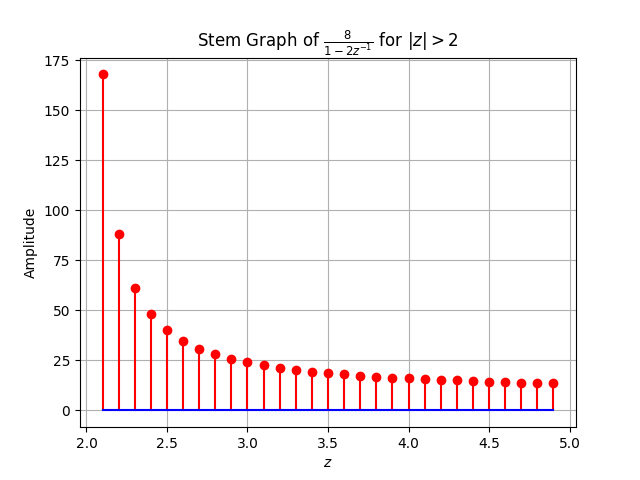
\includegraphics[scale=0.52]{py_11.png}
    \label{fig:enter-label}
\end{figure}
\begin{figure}[h]
    \centering
    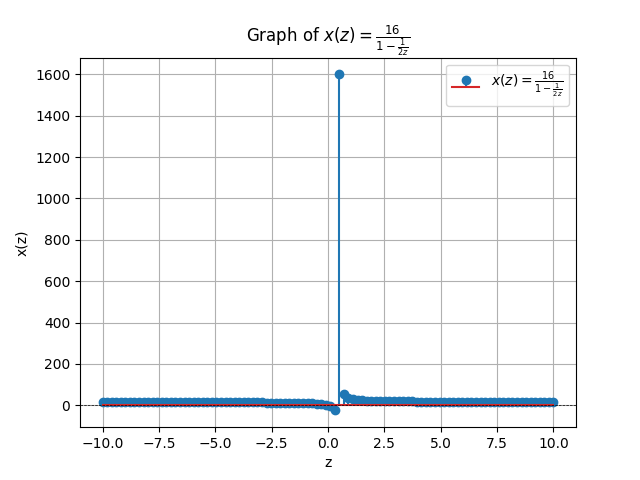
\includegraphics[scale=0.52]{py_12.png}
    \label{fig:enter-label}
\end{figure}
\end{document}
